\documentclass[12pt]{article}
\usepackage{amsmath}
\usepackage{amssymb}
\usepackage[letterpaper,margin=0.85in,centering]{geometry}
\usepackage{fancyhdr}
\usepackage{enumerate}
\usepackage{lastpage}
\usepackage{multicol}
\usepackage{graphicx}

\reversemarginpar

\pagestyle{fancy}
\cfoot{}
\lhead{Math 1560}\chead{Test \# 1 Solutions}\rhead{May 18th, 2017}
%\rfoot{Total: 10 points}
%\chead{{\bf Name:}}
\newcommand{\points}[1]{\marginpar{\hspace{24pt}[#1]}}
\newcommand{\skipline}{\vspace{12pt}}
%\renewcommand{\headrulewidth}{0in}
\headheight 30pt

\newcommand{\di}{\displaystyle}
\newcommand{\abs}[1]{\lvert #1\rvert}
\newcommand{\len}[1]{\lVert #1\rVert}
\renewcommand{\i}{\mathbf{i}}
\renewcommand{\j}{\mathbf{j}}
\renewcommand{\k}{\mathbf{k}}
\newcommand{\R}{\mathbb{R}}
\newcommand{\aaa}{\mathbf{a}}
\newcommand{\bbb}{\mathbf{b}}
\newcommand{\ccc}{\mathbf{c}}
\newcommand{\dotp}{\boldsymbol{\cdot}}
\newcommand{\bbm}{\begin{bmatrix}}
\newcommand{\ebm}{\end{bmatrix}}                   
                  
\begin{document}

%\author{Instructor: Sean Fitzpatrick}
\thispagestyle{fancy}
%\noindent{{\bf Name and student number:}}

 \begin{enumerate}
 \item  Evaluate the following limits:
\begin{enumerate}
 \item $\di \lim_{x\to 3} \frac{x^2-5x+6}{x^2-4x+3}$\points{3} 
\begin{align*}
                   \lim_{x\to 3} \frac{x^2-5x+6}{x^2-4x+3} & = \lim_{x\to 3}\frac{(x-2)(x-3)}{(x-1)(x-3)}\\[10pt]
& = \lim_{x\to 3}\frac{x-2}{x-1}\\[10pt]
& = \frac{3-2}{3-1} = \frac{1}{2}.
                  \end{align*}



\bigskip

 \item  $\di \lim_{x\to 0}\frac{\sin(5x)}{x}$\points{3} 
\begin{align*}
                    \lim_{x\to 0}\frac{\sin(5x)}{x} & = \lim_{x\to 0}5\left(\frac{\sin(5x)}{5x}\right)\\[10pt]
 & = 5\lim_{x\to 0}\frac{\sin(5x)}{5x}\\[10pt]
 & = 5(1) = 1.
                   \end{align*}

\bigskip

 \item $\di \lim_{x\to 0}\left(\frac{1}{x}-\frac{1}{x^2+x}\right)$ \points{3} 
\begin{align*}
                    \lim_{x\to 0}\left(\frac{1}{x}-\frac{1}{x^2+x}\right) & = \lim_{x\to 0}\left(\frac{(x+1)-1}{x(x+1)}\right)\\[10pt]
& = \lim_{x\to 0}\frac{x}{x(x+1)}\\[10pt]
& = \lim_{x\to 0}\frac{1}{x+1}\\[5pt]
& = \frac{1}{0+1} = 1.
                   \end{align*}


\end{enumerate}
\newpage

\item The graph of a function $f$ is given below:

\begin{center}
 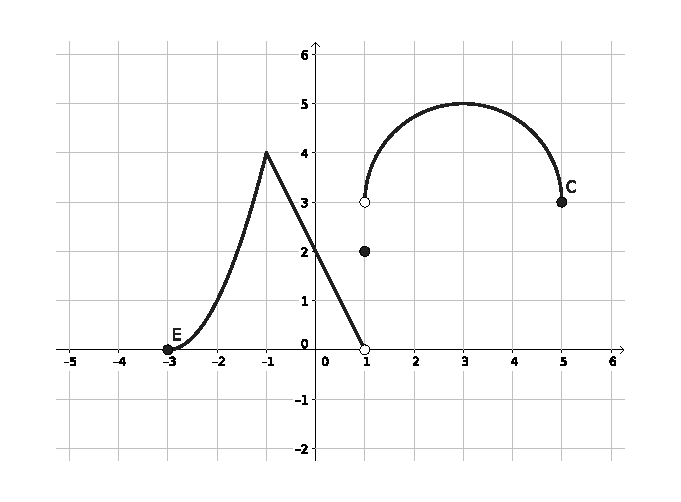
\includegraphics[width=5in]{TT1_fig1}
\end{center}

\begin{enumerate}
 \item What is the domain of $f$?  $\operatorname{dom}(f) = [-3,5]$.\points{1}

\bigskip


 \item $\di\lim_{x \to -1^-}f(x)= $ \underline{\hspace{0.3in}4\hspace{0.3in}} and $\di \lim_{x\to -1^+}f(x)= $ \underline{\hspace{0.3in}4\hspace{0.3in}}  \points{1}

\bigskip




 \item $\di \lim_{x \to 1^-}f(x)=$ \underline{\hspace{0.3in}0\hspace{0.3in}} and $\di \lim_{x\to 1^+}f(x) =$ \underline{\hspace{0.3in}3\hspace{0.3in}} \points{1}

\bigskip



 \item On what interval(s) is $f$ continuous? $[-3,1)$ and $(1,5]$.\points{1}
\end{enumerate}

\bigskip



\item What are the horizontal and vertical asymptotes (if any) of $f(x) = \dfrac{\sqrt{x^2+1}}{x-1}$?\points{2}

\bigskip

There is a vertical asymptote at $x=1$ since $1-1=0$ but $\sqrt{1^2+1} =\sqrt{2}\neq 0$.

We note that
\[
 \dfrac{\sqrt{x^2+1}}{x-1} = \dfrac{\sqrt{x^2(1+1/x^2)}}{x(1-1/x)} = \dfrac{\abs{x}\sqrt{1+1/x^2}}{x(1-1/x)}.
\]
For $x>0$, we have $\abs{x}=x$ and $f(x)=\dfrac{\sqrt{1+1/x^2}}{1-1/x}\to 1$ as $x\to \infty$.

For $x<0$, we have $\abs{x}=-x$ and $f(x) = -\dfrac{\sqrt{1+1/x^2}}{1-1/x}\to -1$ as $x\to \infty$.

Thus, $y=1$ and $y=-1$ are both horizontal asymptotes.
\end{enumerate}





\end{document}